\documentclass[t,9pt,svgnames]{beamer}
\usepackage[latin1]{inputenc}
\usepackage{framed}
\usepackage{graphics}
\usepackage{helvet}
\usepackage{courier}
\usepackage{amsmath}
\usepackage[absolute,overlay]{textpos}
\usepackage{fancybox}
\usepackage{bm} % Use \bm to generate bold math fonts

%%%%% NOTE TO USER %%%%%%%
%
%  This template requires the 'frame-bg.pdf' and 'title-bg.pdf' be found.  It should have been included with
%  this example.
%%%%%%%%%%%%%%%%%%%%%%%%%


\graphicspath{
{figures/}
}

\usetheme{INL}

\usepackage{listings}
\lstset{%
  basicstyle=\ttfamily\tiny,
  frame=single,
  backgroundcolor=\color{cbbkng},
  language={},
  emphstyle={\color{red}},
	showstringspaces=false,
% basicstyle=\scriptsize\ttfamily,
  basicstyle=\small\ttfamily,
  commentstyle=\color{inl@green},
	keywordstyle=\bfseries,
  escapeinside=$$
}

\setbeamercolor{codeboxcolor}{fg=white,bg=black}

\definecolor{bubblebkng}{rgb}{0.98,0.98,0}
%\definecolor{cbbkng}{rgb}{0.98,0.9,0.98}
\definecolor{cbbkng}{RGB}{227,233,252}

\newenvironment{codebox}{}{}
% #1 - width
% #2 - position on the page (<dim>,<dim>)
% #3 - text
\newcommand{\bubbleat}[3]{\begin{textblock*}{#1}[1,1](#2)
\fcolorbox{black}{yellow}{%
\scriptsize\begin{Bcenter}
#3
\end{Bcenter}}
\end{textblock*}}

\newcommand{\uo}{\ensuremath{\mbox{UO}_2}}
\newcommand{\mytilde}{\raise.17ex\hbox{$\scriptstyle\sim$}}

\newcommand{\code}[1]{\texttt{#1}}
\newcommand{\comment}[1]{{\usebeamercolor[fg]{comment code} #1}}

\newenvironment{codelst}{\begin{verbatim}}{\end{verbatim}}

\newcommand{\blue}[1]{{\color{blue}#1}}
\newcommand{\red}[1]{{\color{red}#1}}

% TOC
\newdimen\tocpnumwd
\tocpnumwd=30pt

\makeatletter

\def\dottedtocline#1#2#3{\bgroup%
  \advance\leftskip by #1%
  \advance\rightskip by #2%
  \advance\rightskip by \tocpnumwd%
  \leaders\hbox to 1.5em{\hss .\hss}\hfill\nobreak%
  \rlap{\hbox to \tocpnumwd{\hfil #3}}\par\egroup}

%\def\beamer@sectionintoc #1#2#3#4#5{{\small#2\dottedtocline{7em}{6em}{#3}}\par}
\def\beamer@sectionintoc #1#2#3#4#5{{\hspace{5em}\hyperlink{Navigation#3}{\small#2\dotfill{#3}}\hspace*{4em}}\par}


%\def\beamer@subsectionintoc %#1#2#3#4#5#6{{\small#3\dottedtocline{9em}{6em}{#4}}\par}
\def\beamer@subsectionintoc #1#2#3#4#5#6{{\hspace{6em}\hyperlink{Navigation#4}{\small#3\dotfill{#4}}\hspace*{4em}}\par}

\newcommand{\mytoc}{\@starttoc{toc}}

\makeatother

%This is an ugly hack to fix a bug with Beamer that doesn't put enough vertical
%space above the first list environment in a columns environment when the [t]
%option is passed to the beamer class.  Use this command somewhere in the
%column before using a list or itemize
\newcommand{\vspacehack}{
\setbox0=\vbox{
\begin{itemize}
\item
\end{itemize}
}}


\begin{document}

% user start editing here! %
\title[RAVEN Workshop]{RAVEN Workshop}
\subtitle{Advanced UQ With Collocation Methods}
\institute[INL]{Nuclear Engineering Methods Development Department\\
Idaho National Laboratory}

\begin{titleframe}{RAVEN Workshop}

{\bfseries\emph{Advanced UQ With Collocation Methods}}

\vfill
{\small Nuclear Engineering Methods Development Department\\
Idaho National Laboratory}
\end{titleframe}

\begin{frame}{Table of Contents}
\mytoc
\end{frame}

%
%   OVERVIEW
%
\section{Overview}
\begin{frame}{Overview}
\end{frame}

\begin{frame}{Overview: Session Goal}
  \vfill
  Use advanced methods to accelerate UQ
  \vfill
  \begin{itemize}
    \item For low dimensionality, far fewer runs
  \vfill
    \item For smooth respones, provides accurate ROMs
  \vfill
    \item ROMs contain analytic mean, variance, sensitivities
  \vfill
  \end{itemize}
  \vfill
\end{frame}
%
%   Motivation
%
\section{Motivations}
\begin{frame}{Motivations}
\end{frame}

\begin{frame}{Motivations: Monte Carlo}
  \vfill
  Gold standard in UQ is Monte Carlo, Latin Hypercube
  \vfill
  \begin{itemize}
    \item Consistently convergent (central limit theorem)
  \vfill
    \item Easy to develop
  \vfill
    \item Error diminishes slowly
  \vfill
    \item Requires $1/\epsilon^2$ samples to achieve error $\epsilon$
  \end{itemize}
  \vfill
\end{frame}

\begin{frame}{Motivations: Alternatives to Monte Carlo}
  \vfill
  Some structured samplers can improve greatly on Monte Carlo
  \vfill

  Example: Stochastic Collocation for generalized Polynomial Chaos
  \vfill
  \begin{itemize}
    \item Expand model in orthogonal polynomials
  \vfill
    \item Use integration to determine expansion coefficients
  \vfill
    \item Quadrature methods perform polynomial integrations
  \end{itemize}
  \vfill
  Input dimensions need to be orthogonalized before running
  \vfill
\end{frame}
%
%   Methods
%
\section{Methods}
\begin{frame}{Methods}
\end{frame}

\subsection{Sparse Grid Collocation}
\begin{frame}{Methods: generalized Polynomial Chaos expansion}
  \vfill
  \begin{equation}
    f(x) \approx G(x) = \sum_{k\in\Lambda} c_k \Phi_k(x), 
  \end{equation}
  where
  \begin{itemize}
  \vfill
    \item $f(x)$ is the original model,
  \vfill
    \item $x$ are the uncertain inputs in $f(x)$,
  \vfill
    \item $G(x)$ is the generalized Polynomial Chaos expansion,
  \vfill
    \item $k$ is a multi-index to a polynomial, e.g. (3,1,2),
  \vfill
    \item $\Lambda$ is a pre-determined set of polynomial indices,
  \vfill
    \item $c_k$ are expansion coefficients,
  \vfill
    \item $\Phi_k(x)$ are multidimensional orthogonal polynomials
  \end{itemize}
  \vfill
\end{frame}

\begin{frame}{Methods: gPC Coefficients}
  \vfill
  \begin{equation}
    f(x) \approx G(x) = \sum_{k\in\Lambda} c_k \Phi_k(x), 
  \end{equation}
  \vfill
  $\Phi_k(x)$ are orthogonal,
  \begin{equation}
    c_k = \int_\Omega \rho(x) f(x) \Phi_k(x) dx
  \end{equation}
  where $\rho(x)$ is the joint probability distribution.
  \vfill
  Numerically, use quadratures for $c_k$
  \begin{equation}
    c_k \approx\sum_{\ell=1}^L w_\ell f(x_\ell) \Phi_k(x_\ell))
  \end{equation}
  where $w_\ell$ are the weights and $x_\ell$ are the points
  \vfill
\end{frame}

\begin{frame}{Methods: Large Dimensionality}
  \vfill
  Tensor SCgPC only efficient if $N<4$
  \vfill

  Fight curse of dimensionality using Sparse Grids
  \vfill
  \begin{itemize}
    \item Hyperbolic Cross
    \item Total Degree
  \vfill
    \item Smolyak Quadrature
  \end{itemize}
  \vfill
\end{frame}

\begin{frame}[fragile]{Methods: SCgPC in RAVEN}
  ROM
  \lstinputlisting[basicstyle=\ttfamily\footnotesize,firstline=51,lastline=56,emph={rom,GaussPolynomialRom,y1,y2,ans,TensorProduct}]
          {../../inputs/paul/two/tp2.xml}
  \vfill
  Sampler
  \lstinputlisting[basicstyle=\ttfamily\footnotesize,firstline=35,lastline=44,emph={SparseGridCollocation,sc,y1,uni,y2,rom}]
          {../../inputs/paul/two/tp2.xml}
\end{frame}

\begin{frame}[fragile]{Methods: SCgPC in RAVEN}
  Steps
  %MultiRun
  \lstinputlisting[basicstyle=\ttfamily\footnotesize,firstline=10,lastline=15,emph={sample,sc,poly,collset}]
          {../../inputs/paul/two/tp2.xml}
  %RomTrainer
  \lstinputlisting[basicstyle=\ttfamily\footnotesize,firstline=28,lastline=31,emph={train,collset,rom}]
          {../../inputs/paul/two/tp2.xml}
  %Write Out
  \lstinputlisting[basicstyle=\ttfamily\footnotesize,firstline=20,lastline=23,emph={stats,rom,stats\_tp2}]
          {../../inputs/paul/two/tp2.xml}
\end{frame}


\begin{frame}{Methods: Interpolation Node}
  \vfill
  What if I want to use a different quadrature?
  \vfill

  What if some dimensions require higher-order polynomials than others?
  \vfill

  Specify through an interpolation node
  \lstinputlisting[basicstyle=\ttfamily\footnotesize,firstline=51,lastline=58,emph={Interpolation}]
          {../../inputs/paul/two/td3.xml}
  \vfill
  
\end{frame}

\begin{frame}{Methods: Adaptive}
  \vfill
  What if I don't know what dimensions are higher order?
  \vfill

  Use the Adaptive SCgPC sampler!
  \lstinputlisting[basicstyle=\ttfamily\footnotesize,firstline=35,lastline=50,emph={AdaptiveSparseGrid,Convergence,convergenceStudy}]
          {../../inputs/paul/two/adaptSC.xml}
  \vfill
\end{frame}

\subsection{Sobol Decomposition}
\begin{frame}{Methods: Sobol Decomposition}
\end{frame}

\begin{frame}{Methods: Sobol Decomposition}
  \vfill
  Another kind of expansion
  \begin{align*}
    f(x,y,z) =& f_0 \\
             &+ f_1(x) + f_2(y) + f_3(z)\\
             &+ f_{1,2}(x,y) + f_{1,3}(x,z) + f_{2,3}(y,z) \\
             &+ f_{1,2,3}(x,y,z),
  \end{align*}
  where $f_1(x)=\int\int f(x,y,z)\ dy\ dz$, etc.
  \vfill

  Benefits:
  \vfill
  \begin{itemize}
    \item Many problems dominated by low-order interacations
  \vfill
    \item Provides easy access to Sobol sensitivities
  \vfill
    \item Each sub-term can be modelled as SCgPC ROM
    \begin{itemize}
      \item Most are dimension 2 or less!
    \end{itemize}
  \vfill
    \item Can also be constructed adaptively
    \begin{itemize}
      \item Highest efficiency: Adaptive Sobol with Adaptive SCgPC
    \end{itemize}
  \end{itemize}
  \vfill
\end{frame}

\begin{frame}{Methods: Sobol in RAVEN}
  \vfill
  Sampler
  \lstinputlisting[basicstyle=\ttfamily\footnotesize,firstline=35,lastline=56,emph={AdaptiveSobol,Convergence,convergenceStudy}]
          {../../inputs/paul/two/adaptSobol.xml}
  \vfill
\end{frame}

\begin{frame}{Methods: Sobol in RAVEN}
  \vfill
  ROM
  \lstinputlisting[basicstyle=\ttfamily\footnotesize,firstline=63,lastline=69,emph={HDMRRom,SobolOrder}]
          {../../inputs/paul/two/adaptSobol.xml}
  \vfill
\end{frame}
%
%   Demonstration
%
\section{Demonstration}
\begin{frame}{Demonstration: Attenuation Problem}
\end{frame}

\begin{frame}{Demonstration: the Model}
  \vfill
  \begin{equation}
    f(x) = \prod_{n=1}^N \exp(-x_n/N),
  \end{equation}
  \vfill
  \begin{equation}
    x_n \sim \mathcal{U}(0,1).
  \end{equation}
  \vfill
  Taylor expansion suggests many combinations of high-order terms
  \begin{equation}
    \exp(-x) = 1-x+\frac{x^2}{2!}-\frac{x^3}{3!}+\cdots
  \end{equation}
  \vfill
  Expected: 
  \vfill
  \begin{itemize}
  \vfill
    \item Tensor Product, Total Degree, Adaptive perform well
  \vfill
    \item Hyperbolic Cross should struggle
  \end{itemize}
  \vfill
\end{frame}

\begin{frame}{Demonstration: Attenuation Problem}
  \vfill
  Files:
  \vfill
  \begin{itemize}
    \item \code{hc6.xml}
  \vfill
    \item \code{td3.xml}
  \vfill
    \item \code{tp2.xml}
  \vfill
    \item \code{adaptSC.xml}
  \vfill
    \item \code{adaptSobol.xml}
  \vfill
    \item \code{stats\char`_[case].xml}
  \end{itemize}
  \vfill
\end{frame}

\begin{frame}{Demonstration: Results}
  Two-dimension case
  \begin{columns}
    \begin{column}{0.5\textwidth}
      \begin{figure}
        \centering
        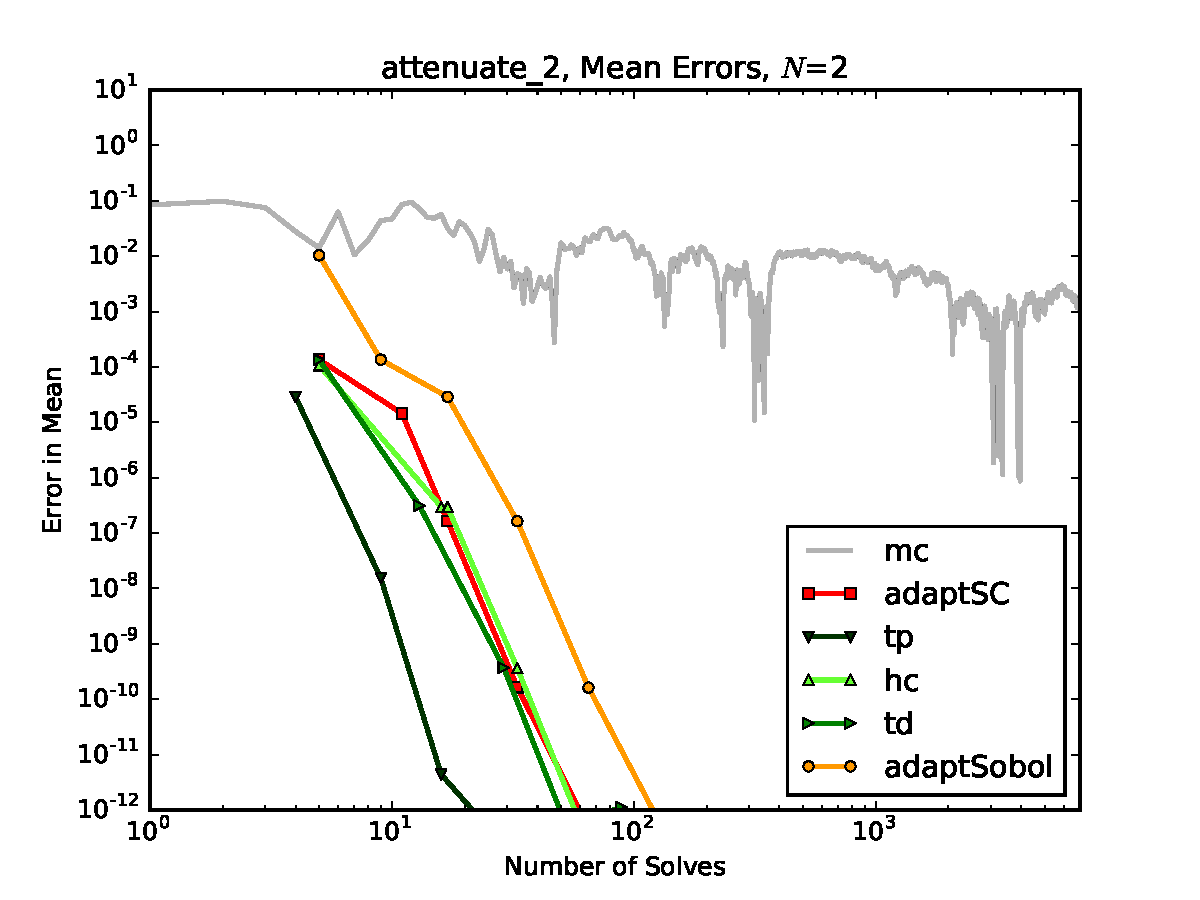
\includegraphics[width=\linewidth]{../../inputs/paul/attenuate_2_mean_errs}
        \caption{Mean, $N=2$}
      \end{figure}
    \end{column}
    \begin{column}{0.5\textwidth}
      \begin{figure}
        \centering
        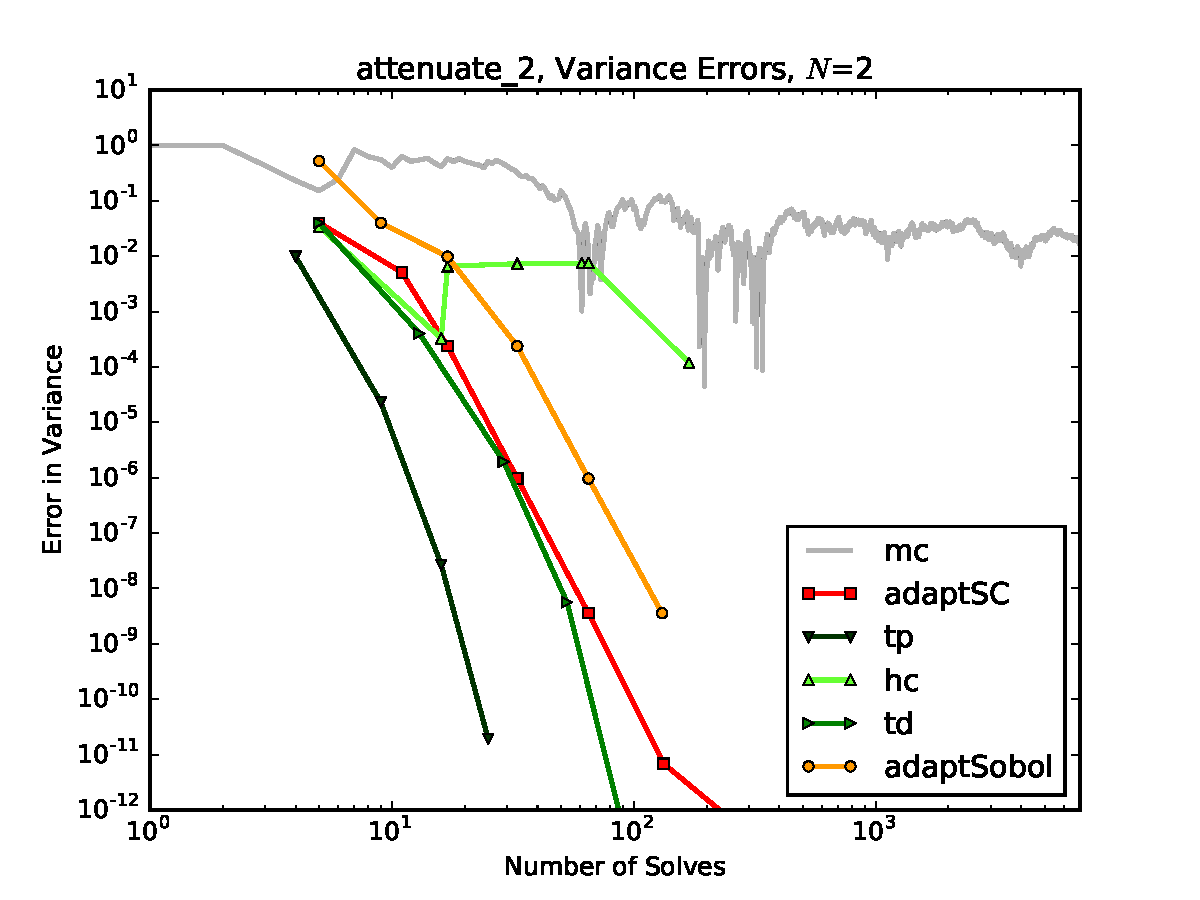
\includegraphics[width=\linewidth]{../../inputs/paul/attenuate_2_variance_errs}
        \caption{Variance, $N=2$}
      \end{figure}
    \end{column}
  \end{columns}
\end{frame}

\begin{frame}{Demonstration: Results}
  Four-dimension case
  \begin{columns}
    \begin{column}{0.5\textwidth}
      \begin{figure}
        \centering
        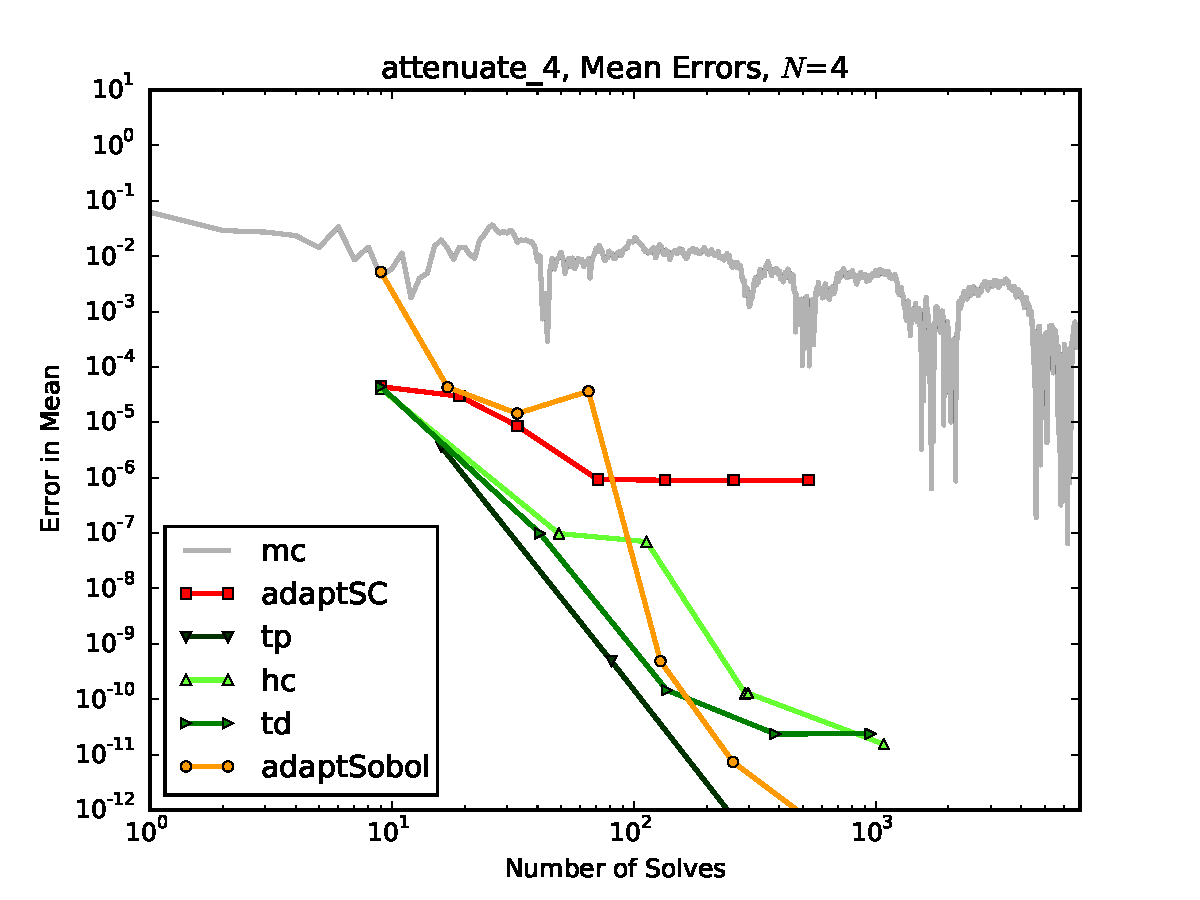
\includegraphics[width=\linewidth]{../../inputs/paul/attenuate_4_mean_errs}
        \caption{Mean, $N=4$}
      \end{figure}
    \end{column}
    \begin{column}{0.5\textwidth}
      \begin{figure}
        \centering
        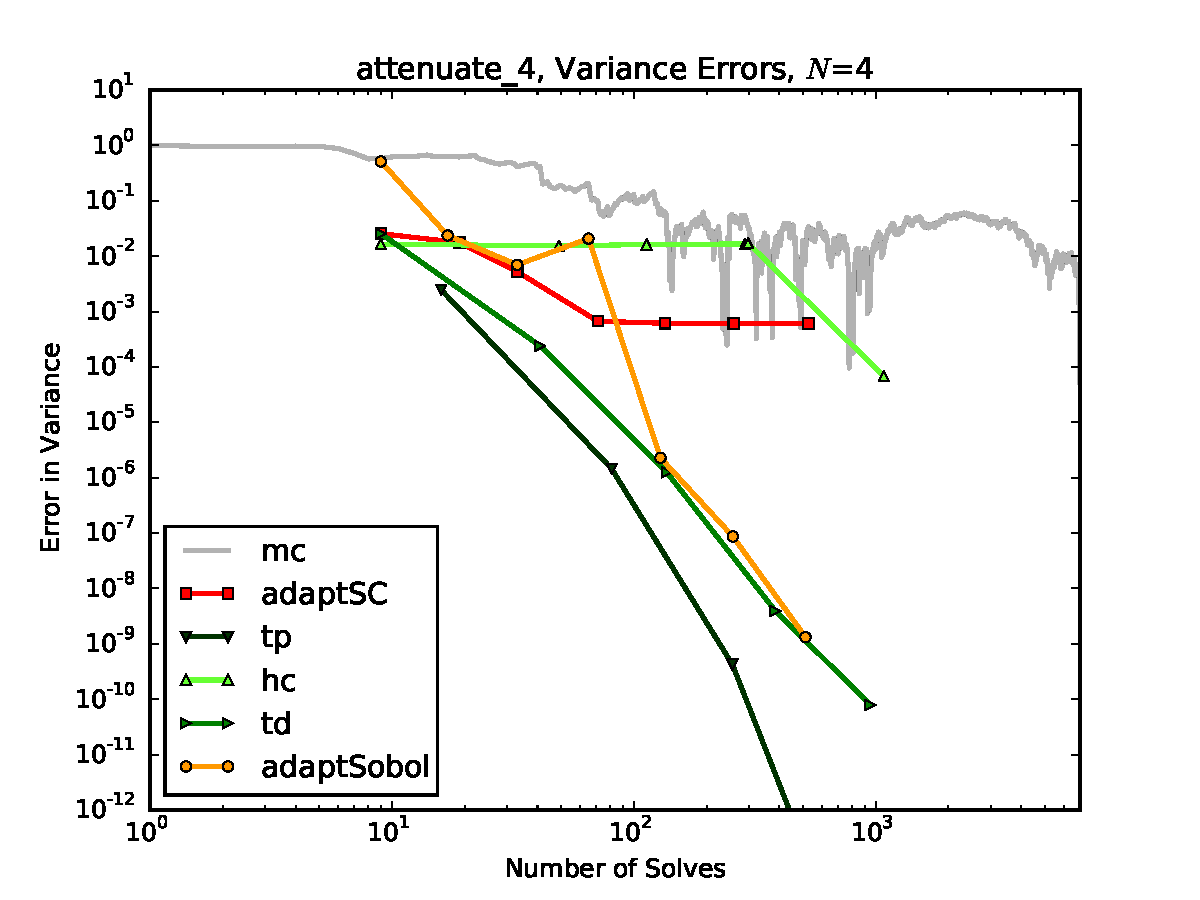
\includegraphics[width=\linewidth]{../../inputs/paul/attenuate_4_variance_errs}
        \caption{Variance, $N=4$}
      \end{figure}
    \end{column}
  \end{columns}
\end{frame}

\begin{frame}{Demonstration: Results}
  Six-dimension case
  \begin{columns}
    \begin{column}{0.5\textwidth}
      \begin{figure}
        \centering
        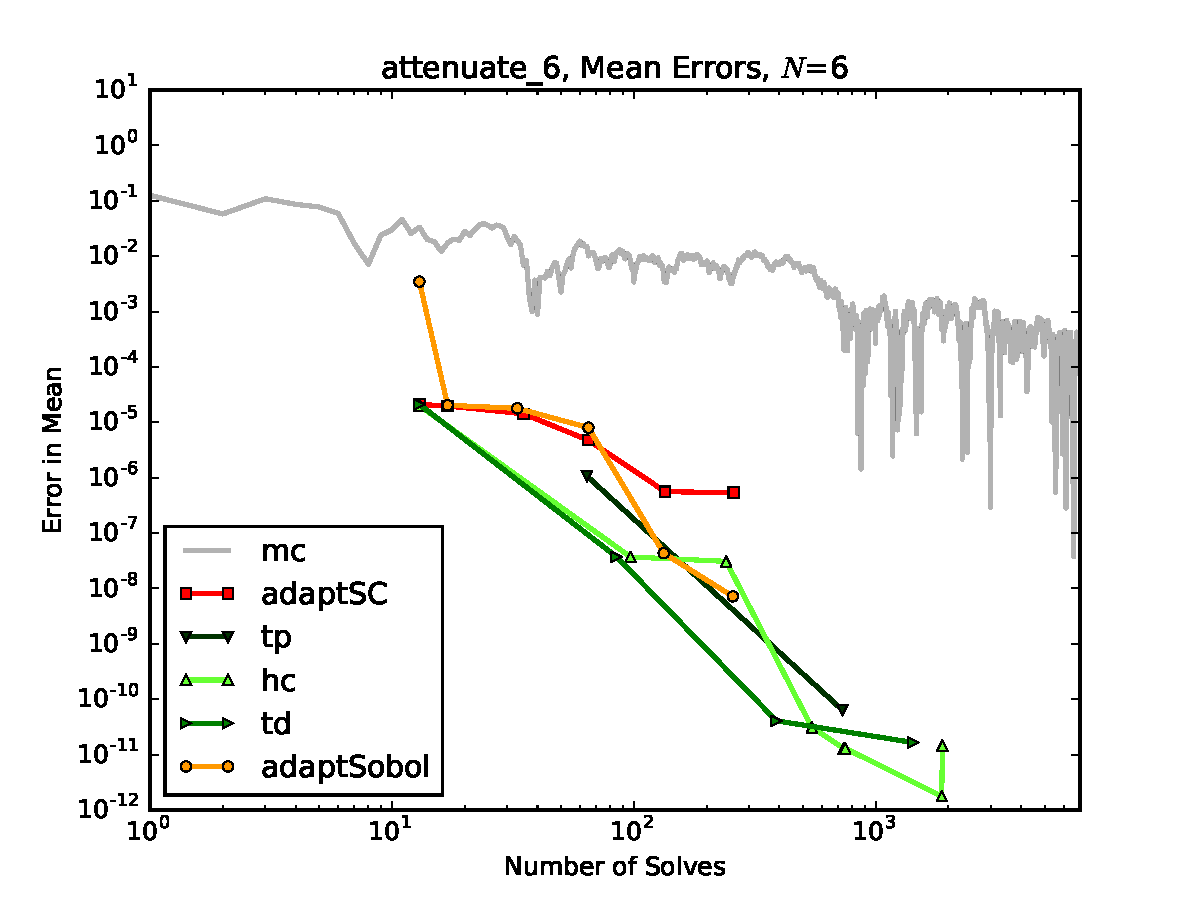
\includegraphics[width=\linewidth]{../../inputs/paul/attenuate_6_mean_errs}
        \caption{Mean, $N=6$}
      \end{figure}
    \end{column}
    \begin{column}{0.5\textwidth}
      \begin{figure}
        \centering
        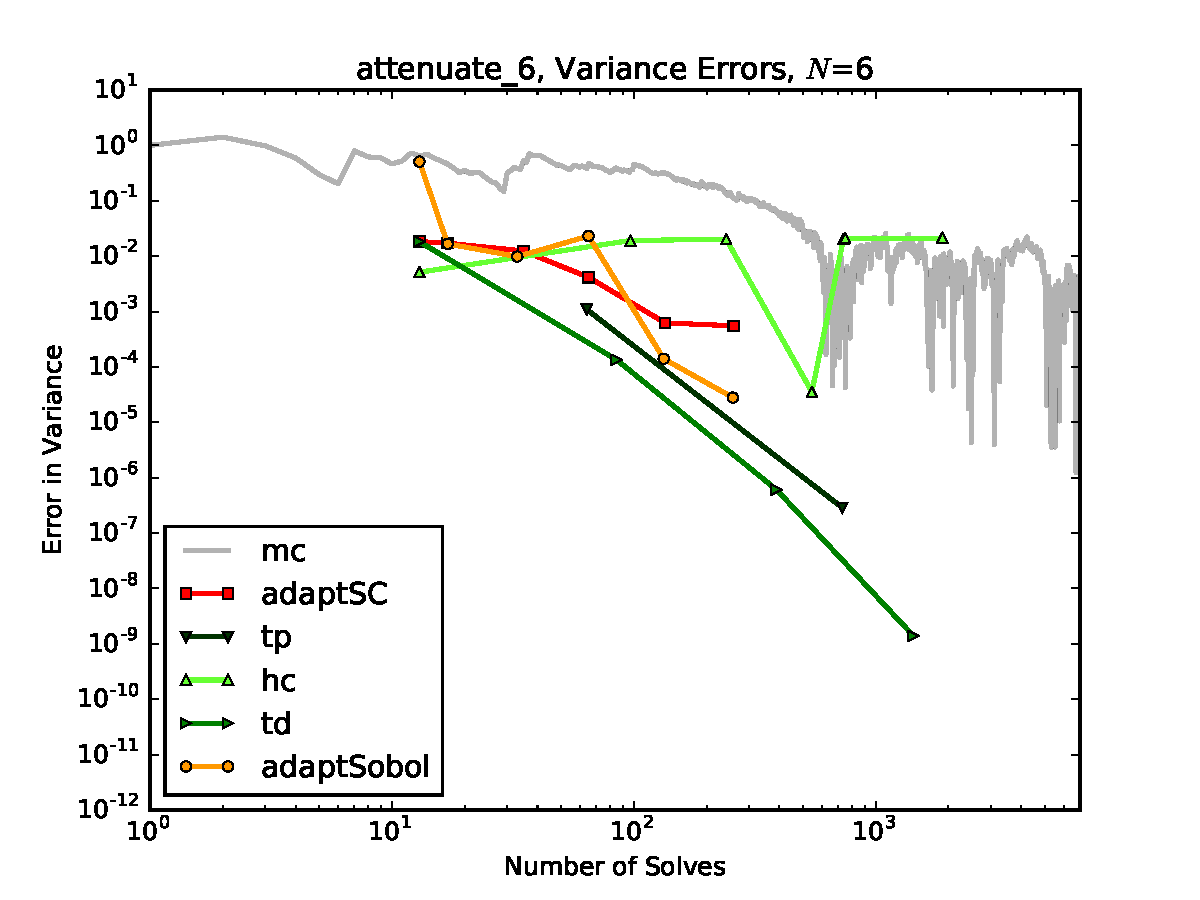
\includegraphics[width=\linewidth]{../../inputs/paul/attenuate_6_variance_errs}
        \caption{Variance, $N=6$}
      \end{figure}
    \end{column}
  \end{columns}
\end{frame}

\begin{frame}{End of Session}
\end{frame}

\begin{frame}{Demonstration: Results}
      \begin{figure}
        \centering
        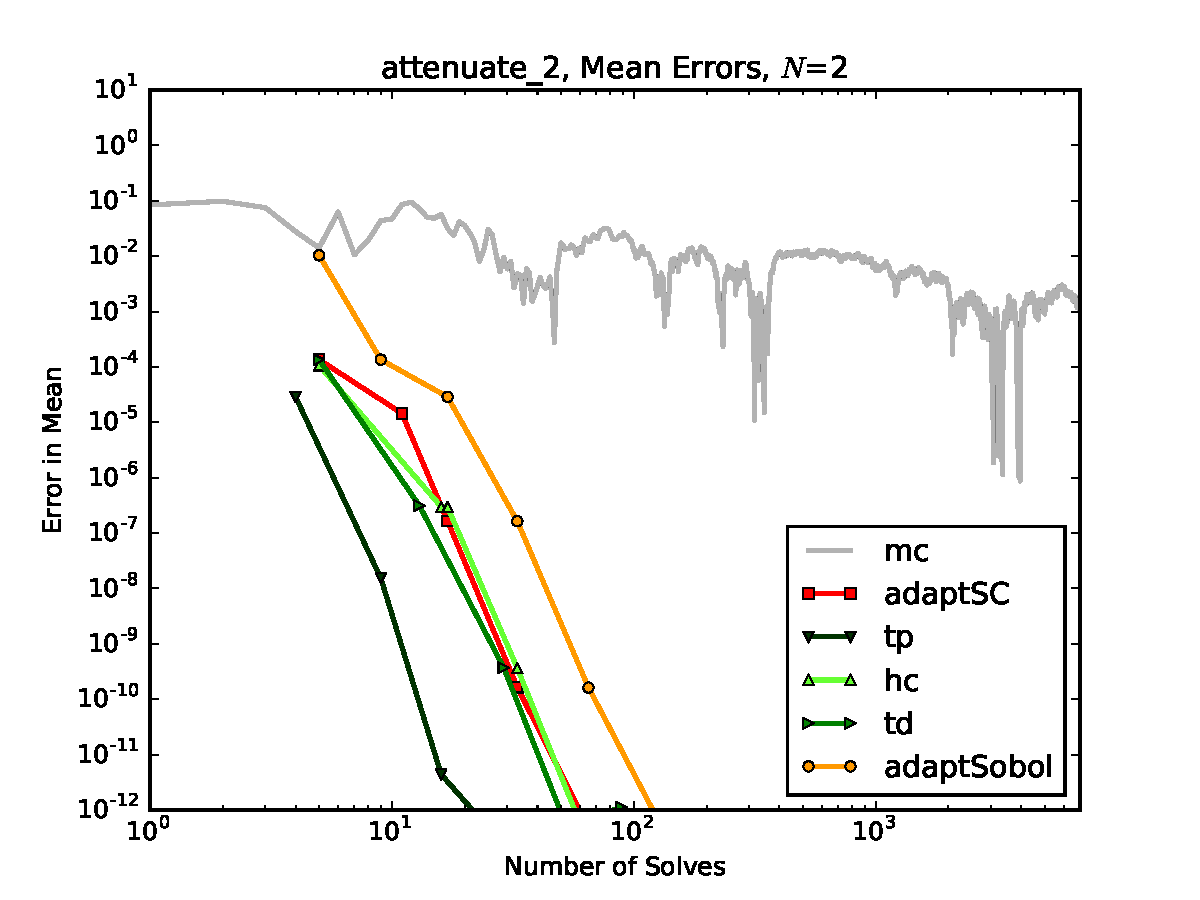
\includegraphics[width=0.8\linewidth]{../../inputs/paul/attenuate_2_mean_errs}
        \caption{Mean, $N=2$}
      \end{figure}
\end{frame}
\begin{frame}{Demonstration: Results}
      \begin{figure}
        \centering
        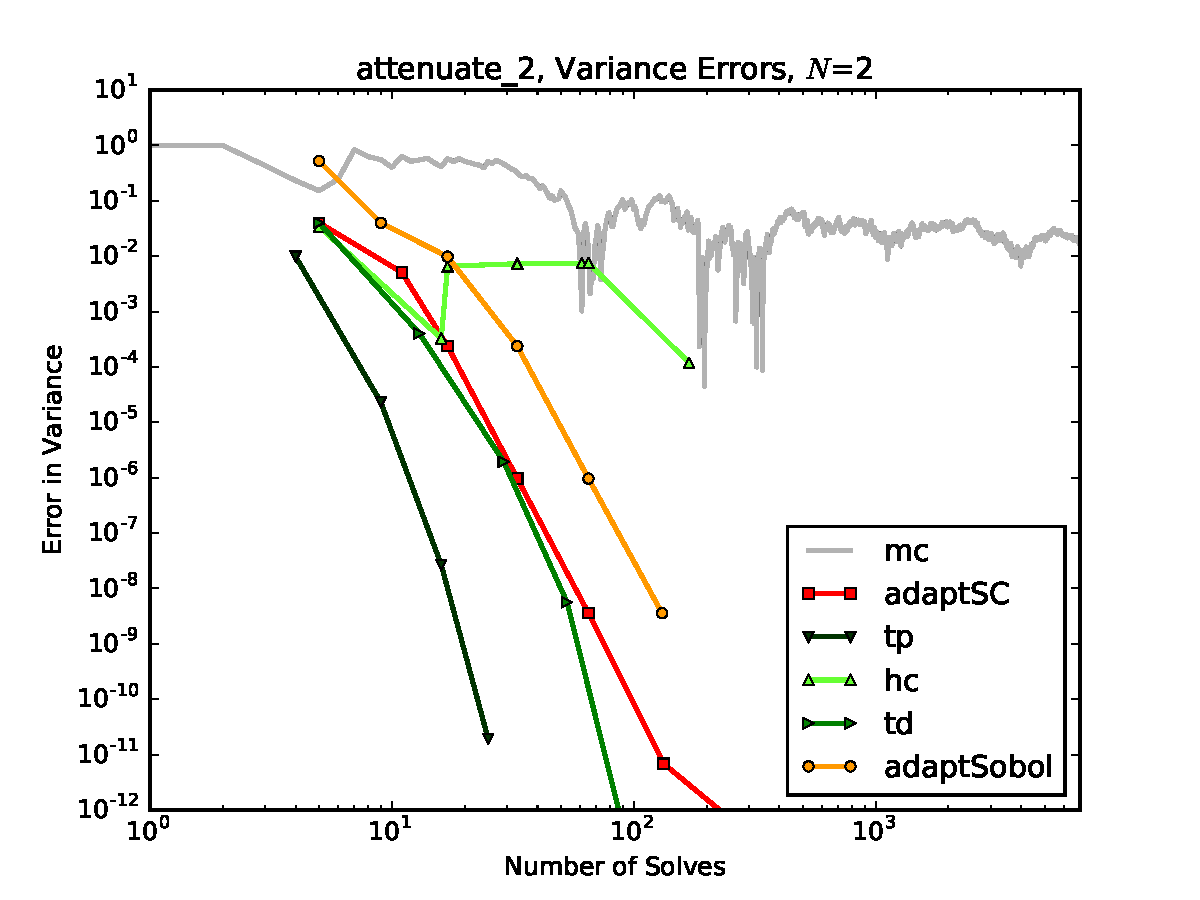
\includegraphics[width=0.8\linewidth]{../../inputs/paul/attenuate_2_variance_errs}
        \caption{Variance, $N=2$}
      \end{figure}
\end{frame}

\begin{frame}{Appendix}
      \begin{figure}
        \centering
        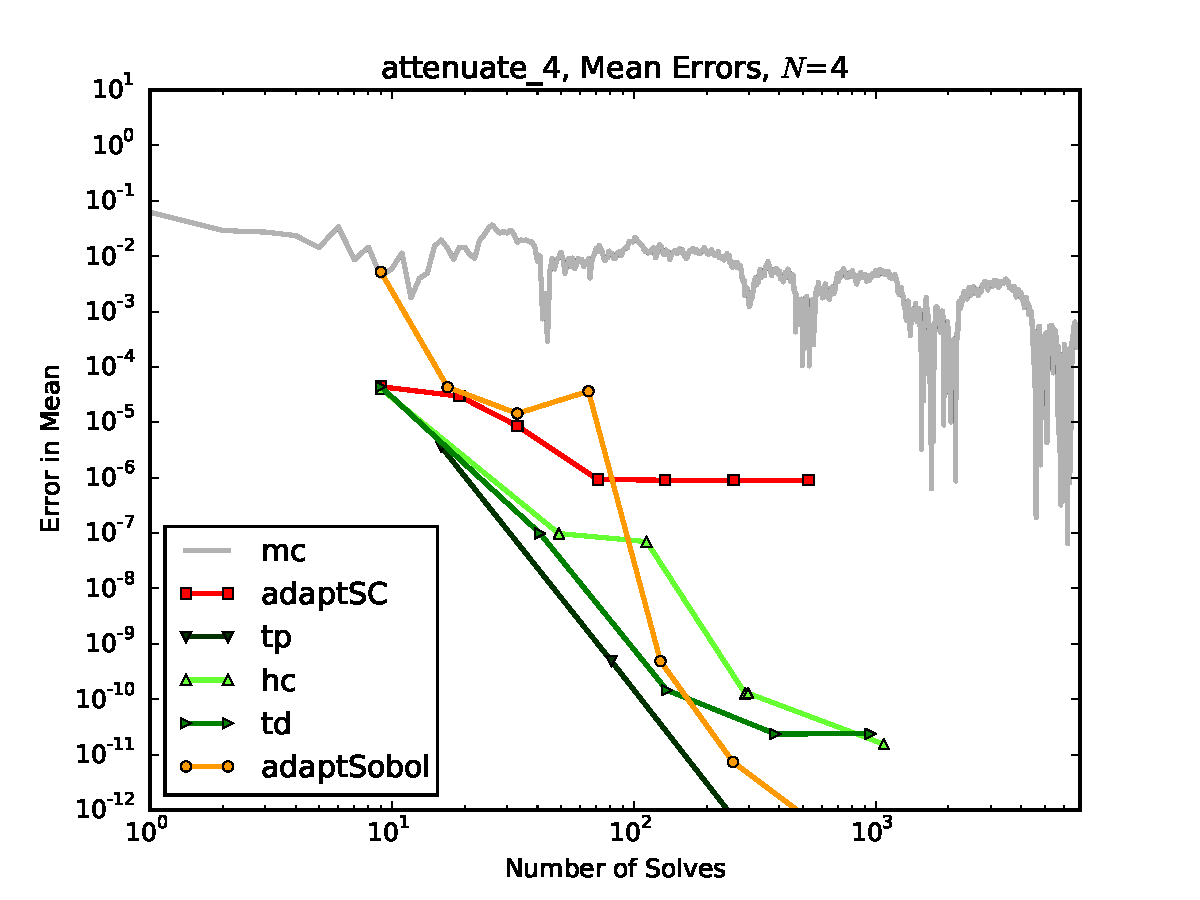
\includegraphics[width=0.8\linewidth]{../../inputs/paul/attenuate_4_mean_errs}
        \caption{Mean, $N=4$}
      \end{figure}
\end{frame}
\begin{frame}{Appendix}
      \begin{figure}
        \centering
        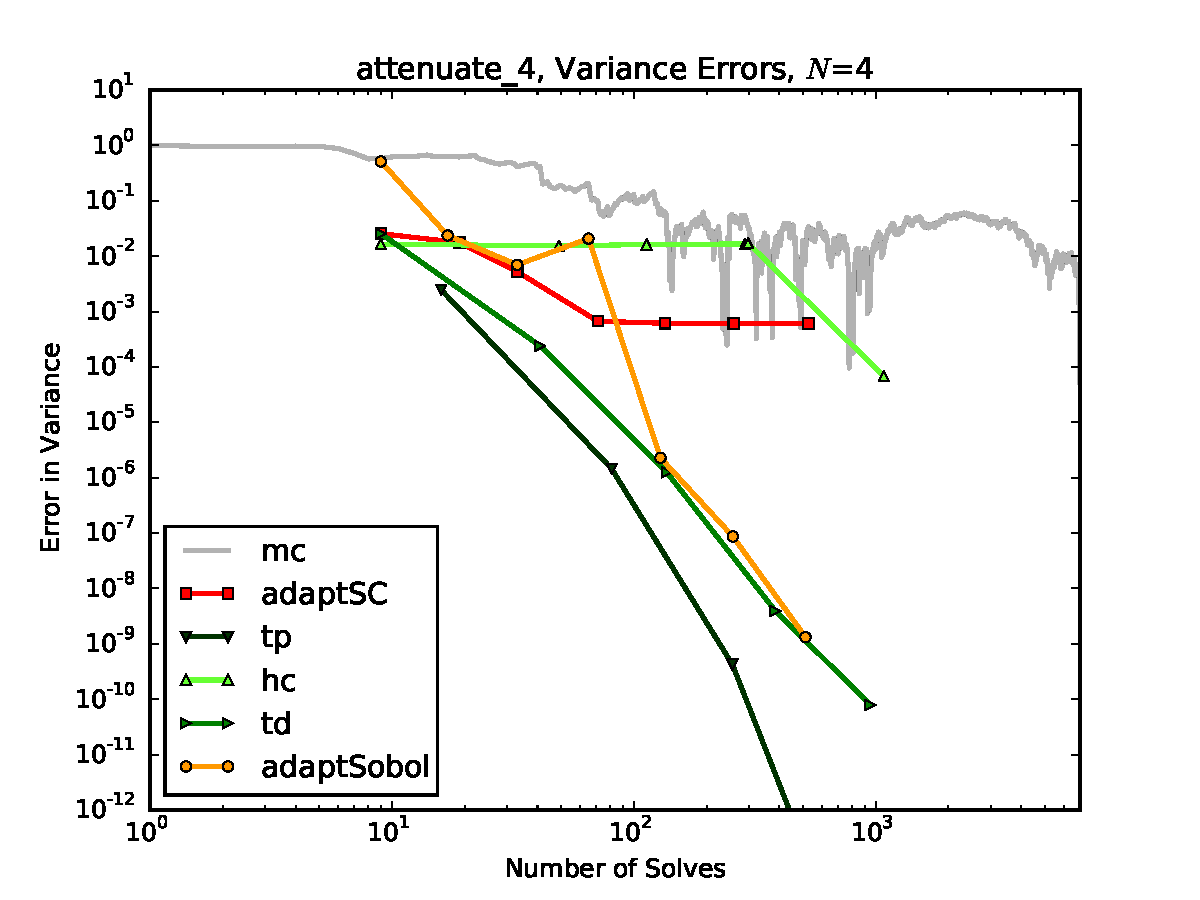
\includegraphics[width=0.8\linewidth]{../../inputs/paul/attenuate_4_variance_errs}
        \caption{Variance, $N=4$}
      \end{figure}
\end{frame}

\begin{frame}{Appendix}
  \begin{figure}
    \centering
    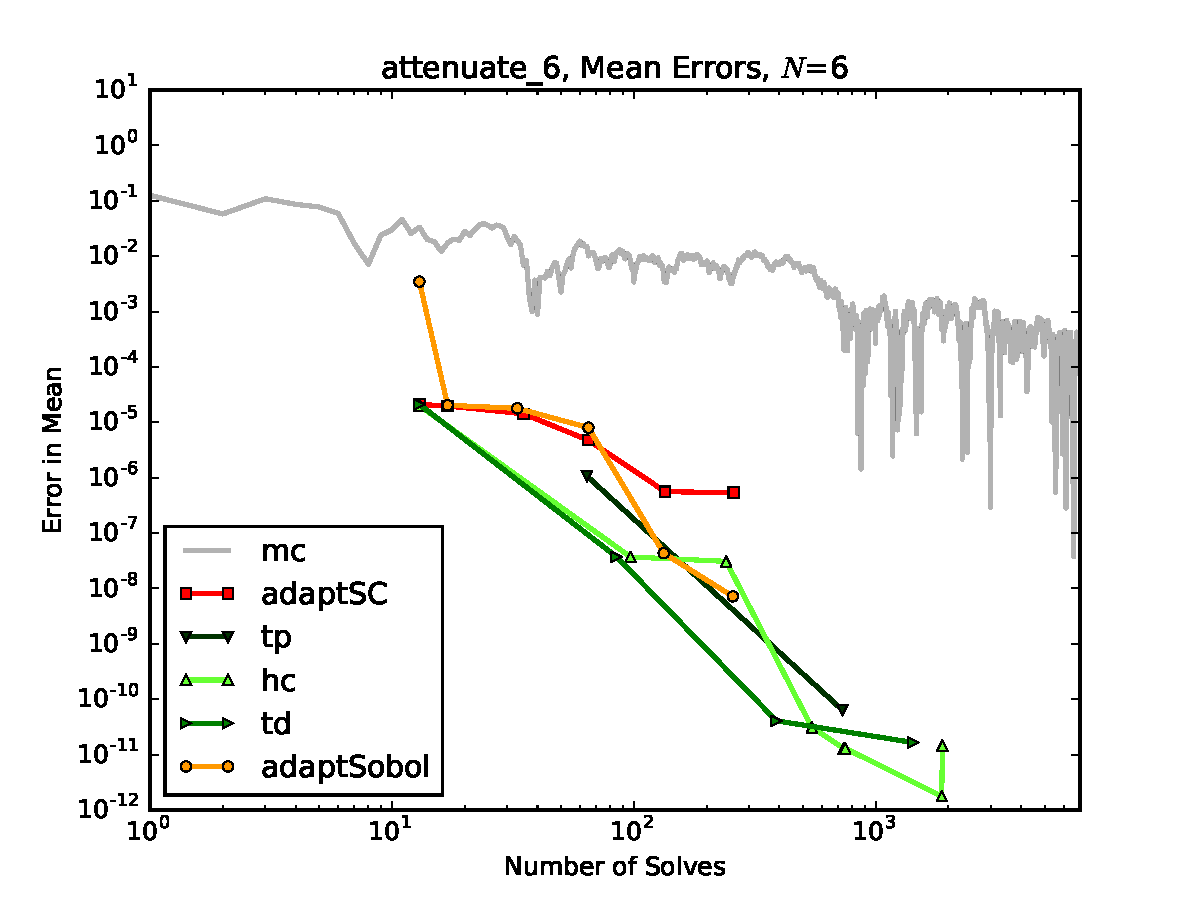
\includegraphics[width=0.8\linewidth]{../../inputs/paul/attenuate_6_mean_errs}
    \caption{Mean, $N=6$}
  \end{figure}
\end{frame}
\begin{frame}{Appendix}
  \begin{figure}
    \centering
    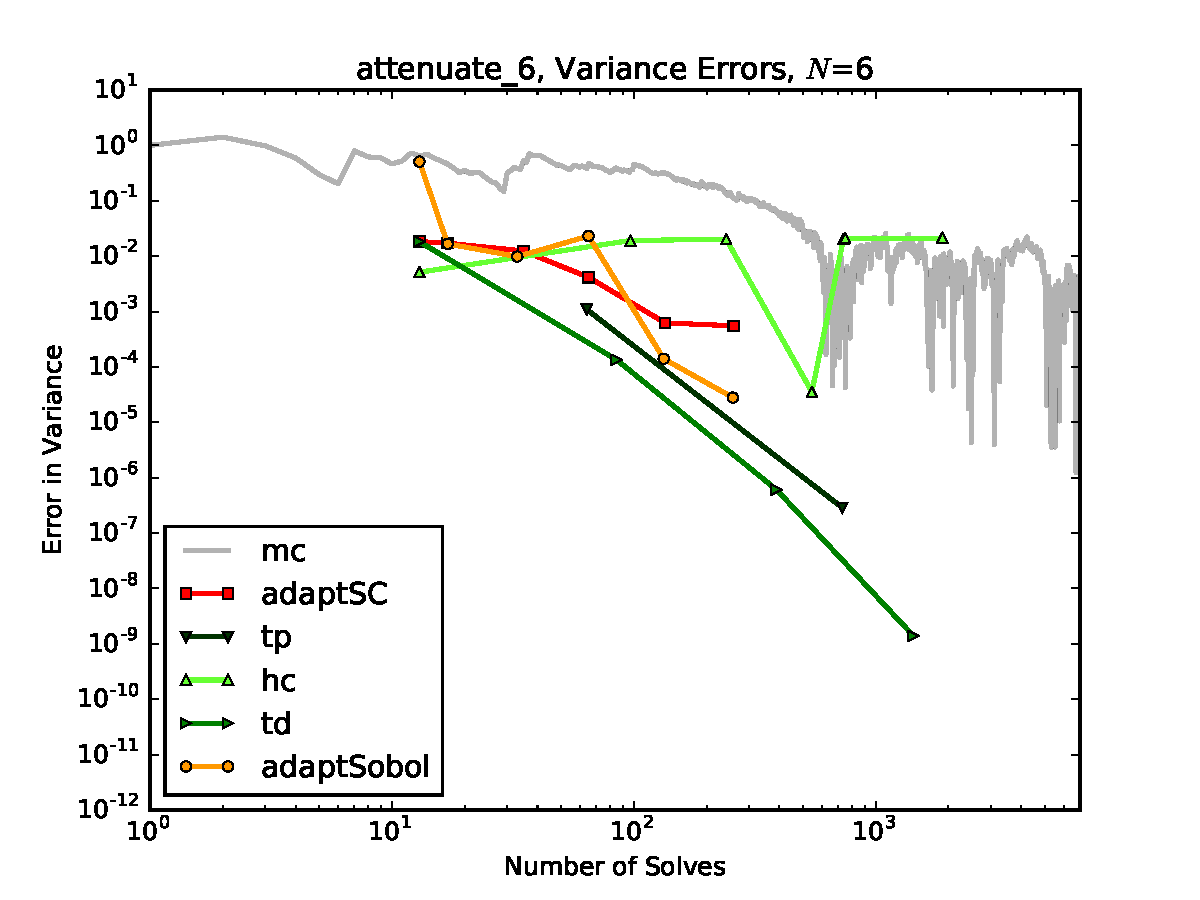
\includegraphics[width=0.8\linewidth]{../../inputs/paul/attenuate_6_variance_errs}
    \caption{Variance, $N=6$}
  \end{figure}
\end{frame}

\end{document}
